\noindent
\begin{description}
\item[Objectif :] savoir coder les nombres, entiers et réels.
\item[Syntaxe \python :] \mbox{}
\begin{Verbatim}
>>> (1000).to_bytes(2, byteorder='big', signed=True)
b'\x03\xe8'
>>> (-1000).to_bytes(2, byteorder='big', signed=True)
b'\xfc\x18'
\end{Verbatim}
\end{description}

\noindent\begin{minipage}{7cm}
\begin{description}
\item[] \mbox{}
\begin{Verbatim}
>>> pi
3.141592653589793
>>> float.hex(pi)
'0x1.921fb54442d18p+1'
>>> float.hex(-pi)
'-0x1.921fb54442d18p+1'
\end{Verbatim}
\end{description}
\end{minipage}
\mbox{}\hfill
\fbox{\begin{minipage}{8cm}\footnotesize
\centerline{codage des nombres réels}
\vspace*{2mm}

\centerline{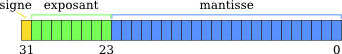
\includegraphics[width=8cm]{IEEE754.png}}
\vspace*{1mm}

\centerline{norme \textsc{Ieee} 754 simple précision}
\centerline{$\pi \rightarrow$ 0 10000000 10010010000111111011011}

\end{minipage}}
%\begin{tabular}{c}
%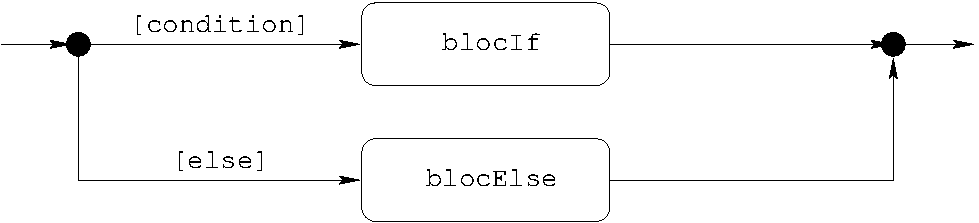
\includegraphics[width=6.5cm]{uml1.pdf}\\[3mm]
%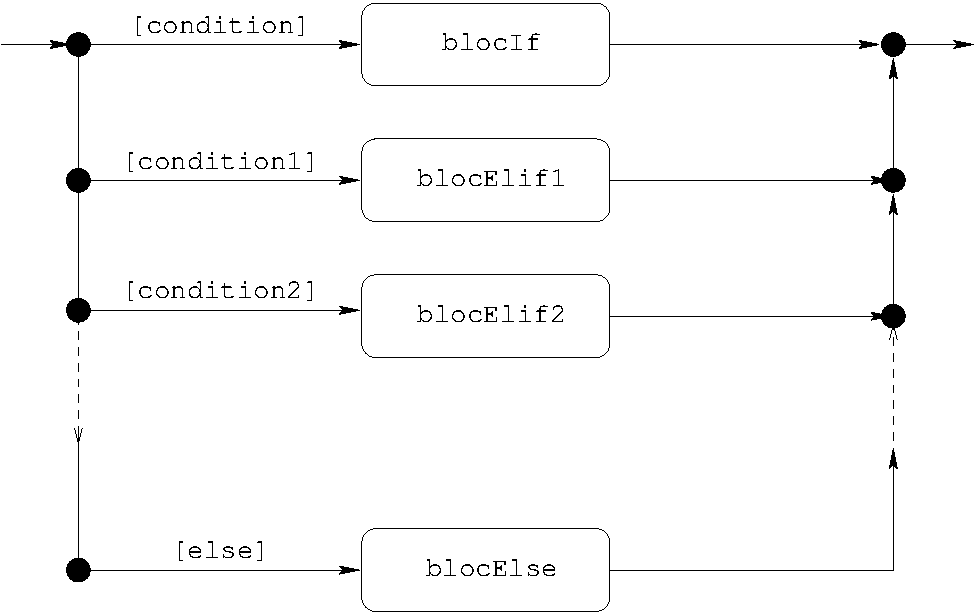
\includegraphics[width=6.5cm]{uml3.pdf}
%\end{tabular}

%-------------------------------------------------------------------------
\subsection{Exemple}
%-------------------------------------------------------------------------

\paragraph{Enoncé :} On cherche à coder un entier dans une base $b$ définie
par $b$ chiffres élémentaires : ici, $b = 16$ (base hexadécimale).

Comme on parle de binaire pour la base 2 ($2^1$), Boby Lapointe (1922-1972, chanteur, féru de mathématiques) proposa 
de dire « bi-binaire » pour la base 4 ($2^2$), et « bi-bi-binaire » 
pour la base 16 ($2^{2^2}$), terme qu'il abrégea en « bibi ».
À partir de ce postulat, Boby Lapointe inventa une notation où à
l'aide de quatre consonnes (B, D, H, K) et de quatre voyelles (A, E, I, O), 
il obtint les seize combinaisons nécessaires et suffisantes pour compter en base « bibi » (16) :
HO (0), HA (1), HE (2), HI (3), BO (4), BA (5), BE (6), BI (7), 
KO (8), KA (9), KE (10), KI (11), DO (12), DA (13), DE (14), DI (15).


%\paragraph{Méthode :} \mbox{}
%
%Et, pour définir un nombre, il suffit d'énumérer les chiffres (en « bibi ») qui le composent.

\paragraph{Questions :} \mbox{}

\begin{question}[« base bibi » : décodage]
Décoder en base décimale l'entier $n = (HIDEKO)_{bibi}$.
\end{question}

\begin{question}[« base bibi » : codage]
Coder en base « bibi » l'entier $n = (538)_{10}$.
\end{question}

%-------------------------------------------------------------------------
\subsection{Généralisation}
%-------------------------------------------------------------------------
Un entier positif en base $b$ est représenté par une suite de
chiffres {$(r_nr_{n-1}\ldots r_1r_0)_b$}
où les $r_i$ sont des chiffres de la base $b$ ($0\leq r_i < b$).
Ce nombre a pour valeur:
$$r_nb^n + r_{n-1}b^{n-1} + \ldots + r_1b^1 + r_0b^0 = \sum^{i=n}_{i = 0} r_ib^i$$
Exemples :
$\displaystyle\begin{array}[t]{llllr}
(123)_{10} &=& 1.10^2 + 2.10^1 + 3.10^0  &=& (123)_{10}\\
(123)_{5}  &=& 1.5^2 + 2.5^1 + 3.5^0     &=&  (38)_{10}\\
(123)_{8}  &=& 1.8^2 + 2.8^1 + 3.8^0     &=&  (83)_{10}\\
(123)_{16} &=& 1.16^2 + 2.16^1 + 3.16^0  &=& (291)_{10}
\end{array}$
\newpage
\begin{question}[codage binaire d'un entier positif]\mbox{}
\begin{enumerate}
\item Décoder en base décimale les nombres binaires suivants :
	$(10110010)_2$, $(00110001)_2$ et $(11011101)_2$.
\item Coder en base 2 les entiers décimaux suivants :
	$(532)_{10}$, $(493)_{10}$ et $(77)_{10}$.
\end{enumerate}

\end{question}

Pour coder les nombres négatifs, une première idée est de réserver un bit pour
le signe, les autres bits représentant la valeur absolue du nombre. 

\begin{question}[nombres relatifs]\label{q-relatifs}\mbox{}
On veut coder un nombre relatif (entier négatif, positif ou nul) sur $k=8$ bits
en réservant le bit le plus à gauche pour le signe ($+ : 0 , - : 1$) et les 7 bits
restant pour coder la valeur absolue du nombre.
\begin{enumerate}
\item Coder l'entier -57 sur 8 bits selon cette méthode.
\item Montrer qu'il y a deux manières possibles de coder 0.
\item Montrer que si l'un des nombres $a$ ou $b$ est négatif,
	alors l'addition binaire $a + b$ ne donne pas le résultat escompté.
\end{enumerate}
\end{question}

Pour remédier aux problèmes précédents, on utilise la représentation en 
« complément à 2 » pour coder un entier relatif $n$ sur $k$ bits.
Les entiers positifs sont représentés comme précédemment : bit de poids fort à 0, 
nombre codé sur $(k-1)$ bits.
Les nombres négatifs sont par contre obtenus en codant sur $k$ bits $(2^k-|n|)$ de la manière suivante :
\begin{itemize}
\item on code la valeur absolue sur $k$ bits puis on inverse les bits un à un 
	(« complément à un~» : les 0 deviennent des 1, les 1 deviennent des 0),
\item on ajoute 1 au résultat (les dépassements à gauche sont ignorés).
\end{itemize}

\begin{question}[complément à 2]\mbox{}
\begin{enumerate}
\item Coder le nombre $n = -41$ en complément à 2 sur 8 bits.
\item Montrer que sur $k$ bits $(n + (-n))$ donne bien 0.
\item Montrer que sur $k$ bits le complément à 2 de $(-n)$ redonne bien $n$ $(n = -(-n))$.
\item Montrer que les deux inconvénients de la méthode précédente (question \ref{q-relatifs} 2. et 3.)
	n'existent plus avec la représentation en complément à 2.
\item Déterminer la plage de valeurs entières possibles lorsqu'un
	entier positif, négatif ou nul est codé en binaire 
	sur $k$ chiffres dans la représentation en complément à 2.
\end{enumerate}
\end{question}

%-------------------------------------------------------------------------
\subsection{Applications}
%-------------------------------------------------------------------------
%\begin{question}[cryptarithmes]\mbox{}
%
%\end{question}
%
%\begin{question}[chiffrement par décalage]\mbox{}
%Rot13
%\end{question}
%
%\begin{question}[codes Ascii]\mbox{}
%Rot13
%\end{question}

\begin{question}[base \textsc{D'ni}]\mbox{}
\textsc{D'ni} est un univers imaginaire sur lequel s'appuient les jeux vidéo 
de la série \textsc{Myst}.
Pour compter, les \textsc{D'ni} utilisent un système quinquévigésimal (base 25).
\begin{enumerate}
\item Décoder en base décimale l'entier $n = (21,17,0,23)_{\mbox{\textsc{D'ni}}}$ exprimé en base
	\textsc{D'ni}.
\item Coder l'entier décimal $n = (3562)_{10}$ en base \textsc{D'ni}.
\end{enumerate}
\end{question}
%-------------------------------------------------------------------------
%\newpage
\subsection{Entraînement}
%-------------------------------------------------------------------------

%-------------------------------------------------------------------------
\subsubsection{Enoncé}
%-------------------------------------------------------------------------

\paragraph{Objectif :} 
Coder un nombre réel $x$ selon la norme \textsc{Ieee} 754 simple précision.

\paragraph{Méthode :} 
Un nombre fractionnaire {$(r_nr_{n-1}\ldots r_1r_0.r_{-1}r_{-2}\ldots)_b$}
({\em nombre avec des chiffres après la virgule})
est défini sur un sous-en\-semble borné, incomplet et fini des rationnels.
Un tel nombre a pour valeur dans la base $b$ :
$${r_nb^n + r_{n-1}b^{n-1} + \ldots + r_1b^1 + r_0b^0 + r_{-1}b^{-1} + r_{-2}b^{-2} + \ldots}$$
En pratique, le {\em nombre de chiffres après la virgule} est limité par la taille physique
en machine.
$${(r_nr_{n-1}\ldots r_1r_0.r_{-1}r_{-2}\ldots r_{-k})_b = \sum_{i=-k}^{i=n} r_ib^i}$$

%Un nombre $x$ pourra être représenté en base $b$ par un triplet
%$[s,m,p]$ tel que ${x = (-1)^s \cdot m \cdot b^p}$ où $s$ représente le signe de $x$,
%$m$ sa mantisse et $p$ son exposant ($p$ comme puissance) où :
%\begin{itemize}
%\item signe $s$ : $s = 1$ si $x < 0$ et $s = 0$ si $x \geq 0$
%\item mantisse $m$ : $m \in [1,b[$ si $x \neq 0$ et $m = 0$ si $x = 0$
%\item exposant $p$ : $p \in [min,max]$
%\end{itemize}

Selon la norme \textsc{Ieee} 754 simple précision, un nombre $x$ pourra être représenté 
en base $b$ par un triplet $[s,m,e]$ tel que 
$\displaystyle x = (-1)^s\cdot(1.m)\cdot2^{e-127}$ 
où $s$ représente le signe de $x$, $m$ sa mantisse normalisée et 
$e = p+127$ son exposant $p$ décalé de 127 :
\begin{itemize}
\item signe $s$ : $s = 1$ si $x < 0$ et $s = 0$ si $x \geq 0$
\item mantisse $m' = 1.m$ : $m' \in [1,b[$ si $x \neq 0$ et $m' = 0$ si $x = 0$
\item exposant $p$ : $p \in [min,max]$
\end{itemize}

$$\begin{tabular}{|c|c|c|}
%\hline
%\multicolumn{3}{|c|}{32 bits}\\
\hline
\multicolumn{3}{|c|}{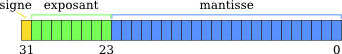
\includegraphics[width=8cm]{IEEE754.png}}\\
\hline
signe & exposant & mantisse normalisée \\
$s$   & $e = p + 127$      & $m$ \\
\hline
1 bit & 8 bits   & 23 bits \\
\hline
\end{tabular}$$

Il s'agira donc de déterminer successivement le signe $s$ de $x$, les parties entière 
et fractionnaire de $|x|$ pour déterminer la mantisse $m$ et l'exposant $p$ associés.

Exemple : $x=-393.0625 = - (1.100010010001)_2 \cdot 2^8$, d'où $s = 1$, $p = 8$,
$e = p + 127 = 135 = (10000111)_2$ et $m' = 1.m = (1.100010010001)_2$, soit
selon la norme \textsc{Ieee} 754 simple précision (32 bits) :
$x = |s|e|m| = |1|10000111|10001001000100000000000|$.

\paragraph{Vérification :} On vérifiera selon deux méthodes :
\begin{enumerate}
\item en recalculant $x$ par la formule $\displaystyle x = (-1)^s\cdot(1.m)\cdot2^{e-127}$ ;
\item en consultant le site \href{http://babbage.cs.qc.edu/IEEE-754/Decimal.html}{\texttt{http://babbage.cs.qc.edu/IEEE-754/Decimal.html}} .
\end{enumerate}

%-------------------------------------------------------------------------
\subsubsection{Exemple}
%-------------------------------------------------------------------------

\paragraph{Enoncé :} Soit à coder le réel $x = -41.3125$ selon la norme 
\textsc{Ieee} 754 simple précision.

\paragraph{Méthode :} Déterminer par étapes successives 
le signe $s$ de $x$, les codes binaires de la partie entière et de
la partie fractionnaire de $|x|$, 
la mantisse $m$ normalisée ($m' = 1.m \in [1,2[$) et l'exposant $e$ relatif à 127.

\paragraph{Résultat :} Selon les recommandations précédentes, 
le codage de $x = -41.3125$ en base $b = 2$ s'effectuera en 5
étapes :
\begin{enumerate}
\item coder le signe de $x$ : $x = -41.3125 < 0 \Rightarrow {s = 1}$
\item coder la partie entière de $|x|$ : {$41 = (101001)_2$}
\item coder la partie fractionnaire de $|x|$ : {$0.3125 = (0.0101)_2$}
\item déterminer la mantisse $m$ normalisée ($1.m \in [1,2[$) : \\
	$|x| = (101001.0101)_2 = (1.010010101)_2\cdot 2^5 \Rightarrow 1.m = (1.010010101)_2
	\Rightarrow m = (010010101)_2$
\item déterminer l'exposant $e$ relatif à 127 :
	$e = 127 + 5 = 132 = (10000100)_2$
\end{enumerate}
Ainsi, selon la norme \textsc{Ieee} 754 simple précision, 
le réel $x = -41.3125$ se code sur 32 bits de la manière suivante :
$$x = -41.3125 = |1|10000100|01001010100000000000000|$$

\paragraph{Vérifications :} on vérifie selon deux méthodes :
\begin{enumerate}
\item en recalculant $x$ par la formule $\displaystyle x = (-1)^s\cdot 1.m \cdot2^{e-127}$ :

\begin{Verbatim}
>>> m = 2**(-2) + 2**(-5) + 2**(-7) + 2**(-9)
>>> e = 132
>>> s = (-1)**1
>>> x = s * (1+m) * 2**(e-127)
>>> x
-41.3125
\end{Verbatim}

Le décodage des 32 bits redonne bien $x = -41.3125$.
\item en consultant le site \href{http://babbage.cs.qc.edu/IEEE-754/Decimal.html} :
	{\texttt{http://babbage.cs.qc.edu/IEEE-754/Decimal.html}} .

$$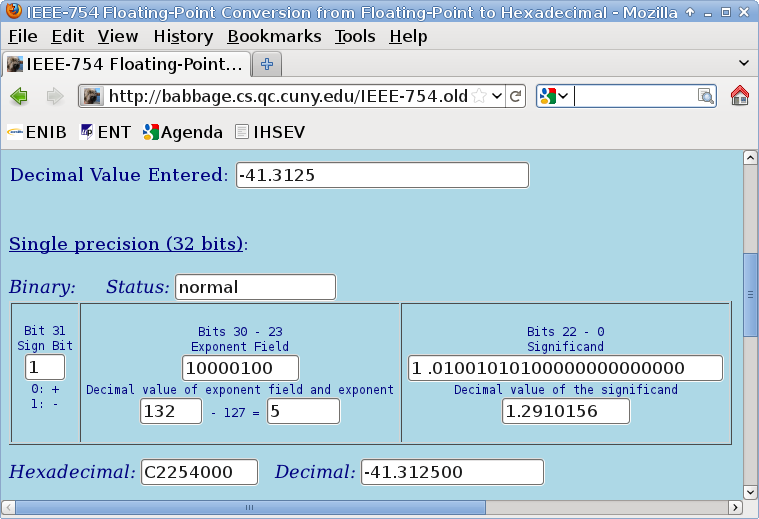
\includegraphics[width=10cm]{ieee-754.png}$$
Le site consulté donne bien le même résultat : \\
$x = -41.3125 = |s|e|m| = |1|10000100|01001010100000000000000|$.
\end{enumerate}

%-------------------------------------------------------------------------
\subsubsection{Questions}
%-------------------------------------------------------------------------
Coder les nombres réels suivants selon la norme \textsc{Ieee} 754 simple précision.
\vspace*{3mm}


\noindent\begin{minipage}{7cm}
\begin{enumerate}
\item $x = 43.1875$
\item $x = -13.0625$
\item $x = 71.25$
\item $x = -54.375$
\item $x = 27.75$
\item $x = -33.625$
\item $x = 69.5$
\item $x = -83.125$
\item $x = 99.3125$
\item $x = -87.5625$
\item $x = 75.875$
\item $x = -61.25$
\end{enumerate}
\end{minipage}
\hfill
\begin{minipage}{7cm}
\begin{enumerate}\setcounter{enumi}{12}
\item $x = -37.03125$
\item $x = 49.1875$
\item $x = -53.0625$
\item $x = 65.25$
\item $x = -77.375$
\item $x = 89.75$
\item $x = -99.625$
\item $x = 7.5$
\item $x = -19.125$
\item $x = 29.3125$
\item $x = -37.5625$
\item $x = 45.875$
\end{enumerate}
\end{minipage}

%-------------------------------------------------------------------------
\subsection{Révisions}
%-------------------------------------------------------------------------

$$\begin{tabular}{|ll@{ : }l|}
\hline
\textbf{Cours} & \cite{cours} & chapitre 3, section 3.1 \\
\textbf{TD}    & \cite{td}    & exercices 1.28, 3.2 à 3.4, 3.20 à 3.22 \\
\hline
\end{tabular}$$
